\documentclass[onecolumn]{article}
\usepackage{amsmath}
\usepackage{enumerate}
\usepackage{enumitem}
\usepackage{listings}
\usepackage[utf8]{inputenc}
\usepackage{amssymb}
\usepackage{tabularx}
\usepackage{tikz}
\usetikzlibrary{arrows,positioning,shapes.geometric}
\usepackage{booktabs}
\usepackage{multirow}
\usepackage{siunitx}
\usepackage{graphicx}
\def\inputGnumericTable{}
\usepackage{fullpage}
\usepackage{color}
\usepackage{array}
\usepackage{longtable}
\usepackage{calc}
\usepackage{multirow}
\usepackage{hhline}
\usepackage{ifthen}
\graphicspath{{./images/}}
\usepackage[big]{titlesec}
\usepackage{titlesec}

\titleformat*{\section}{\huge\bfseries}
\titleformat*{\subsection}{\huge\bfseries}
\titleformat*{\subsubsection}{\huge\bfseries}
\lstset{
    frame=single,
    breaklines=true
}
\usepackage{hyperref}
\usepackage[a3paper,outer=1.5cm,inner=1.5cm,top=1.75cm,bottom=1.5cm]{geometry}
\def\mytitle{\textbf{DEMODULATION TECHNIQUES}}
\def\myauthor{DUDEKULA USENI}
\def\contact{r171099@rguktrkv.ac.in}

\def\contact{r171099@rguktrkv.ac.in }
\def\mymodule{Future Wireless Communication (FWC)}

%\thiswatermark{\centering \put(-15,-100.0){\includegraphics[scale=0.4]{iith.png}} }
\title{\mytitle}
\author{\myauthor\hspace{1em}\\\contact\ FWC22098 -\hspace{0.5em}IITH \hspace{0.5em}\mymodule\hspace{6em}}

\providecommand{\mbf}{\mathbf}
\newcommand{\myvec}[1]{\ensuremath{\begin{pmatrix}#1\end{pmatrix}}}
\providecommand{\qfunc}[1]{\ensuremath{Q\left(#1\right)}}
\providecommand{\cbrak}[1]{\ensuremath{\left\{#1\right\}}}
\providecommand{\brak}[1]{\ensuremath{\left(#1\right)}}
\providecommand{\lsbrak}[1]{\ensuremath{{}\left[#1\right.}}
\providecommand{\rsbrak}[1]{\ensuremath{{}\left.#1\right]}}
\providecommand{\rcbrak}[1]{\ensuremath{\left.#1\right\}}}
\providecommand{\lcbrak}[1]{\ensuremath{\left\{#1\right.}}
\providecommand{\sbrak}[1]{\ensuremath{{}\left[#1\right]}}

\begin{document}
\maketitle
\begin{enumerate}
\begin{Large}


\section{what is Demodulation}
\item[\textbf{}] 

Demodulation is the process of extracting the original information or baseband signal from a modulated carrier signal.The purpose of demodulation is to retrieve the modulating signal, which could be analog or digital data, audio, video, or other forms of information. Demodulation is essential in various communication systems such as radio, television, cellular networks, and wireless data transmission.
\end{Large}\\

\begin{figure}[!h]%
\centering%
%\rule{30pt}{20pt}%
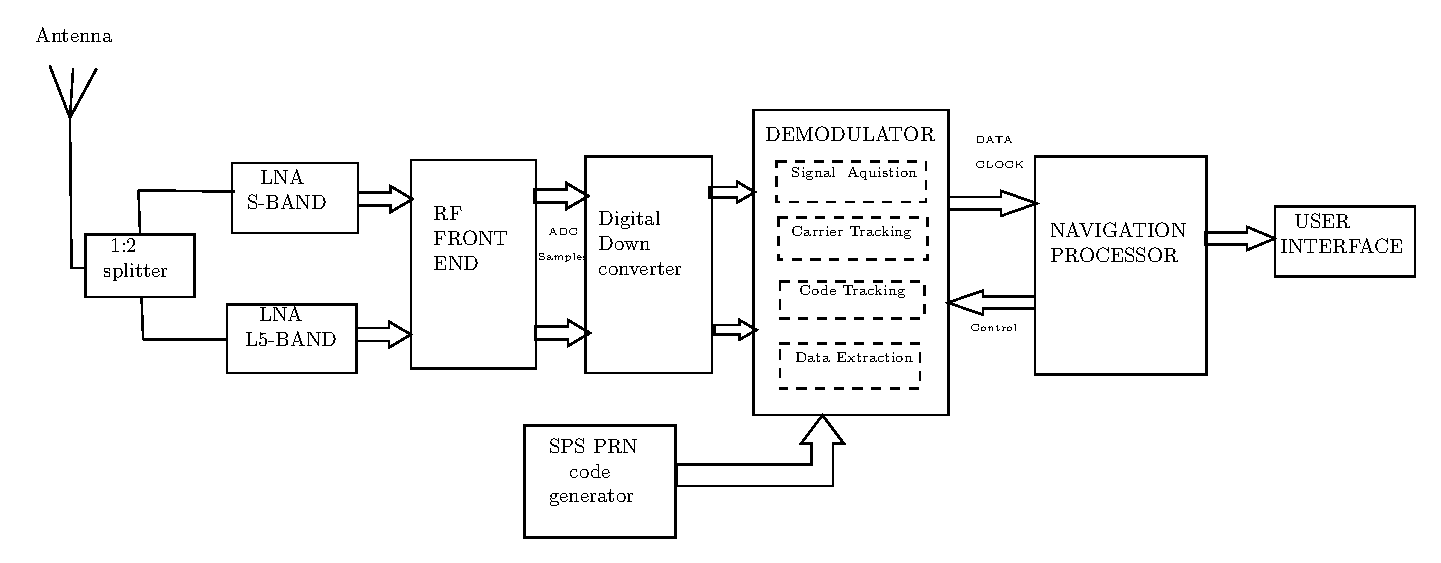
\includegraphics{figures/block1}
\end{figure}
\begin{Large}
\begin{center}
Figure1 : The Block Level Architecture
\end{center}

The demodulation code used in NavIC may vary depending on the specific implementation and receiver hardware. However, I can provide you with a general outline of the demodulation process for NavIC signals.

NavIC signals are transmitted in the L5 frequency band (1176.45 MHz) using BPSK modulation for the navigation message and various modulation schemes (such as BOC and MBOC) for the ranging signal. The demodulation process typically involves the following steps:

\textbf{Signal Acquisition:} The receiver searches for and acquires the NavIC signal by correlating the received signal with a locally generated replica of the spreading code used by the satellites. This process helps in identifying the presence of the NavIC signal and estimating the initial timing offset.

\textbf{Carrier Tracking:} Once the signal is acquired, the receiver performs carrier tracking to estimate and track the carrier frequency and phase of the received signal. This is crucial for demodulation as it ensures accurate demodulation of the navigation message and ranging signal.

\textbf{Code Tracking:} The receiver performs code tracking to estimate and track the spreading code used by the satellites. This helps in maintaining synchronization with the transmitted signal and extracting the navigation data and ranging information.

\textbf{Demodulation:} After carrier and code tracking, the receiver applies the appropriate demodulation technique based on the modulation scheme used for the ranging signal (e.g., BOC, MBOC). This involves extracting the navigation data and ranging information by demodulating the received signal using the corresponding demodulation algorithm.

\textbf{Data Extraction:} Once the demodulation is performed, the receiver extracts the navigation data from the demodulated signal. The navigation data includes information such as satellite ephemeris, clock correction, and other parameters necessary for calculating the receiver's position, velocity, and timing.

\section{Types of Demodulation techniques}
NavIC (Navigation with Indian Constellation), also known as the Indian Regional Navigation Satellite System (IRNSS), is the navigation satellite system developed by the Indian Space Research Organization (ISRO). It uses a variety of demodulation techniques to extract navigation data from the received signals. 
Here are some of the demodulation techniques used in NavIC
\subsection{Binary Phase Shift Keying (BPSK)}
BPSK is a digital modulation scheme that uses two phases, 0 and 180 degrees, to represent binary data. In NavIC, BPSK is used for transmitting the navigation message.
Navigation information constituting Ephemeris and Almanac
data that describes orbital motion and position of satellites in
orbits is a 50 Hz navigation data, encrypted by CA (Course
acquisition) code which has chipping rate of 1.023MHz.
Further it is BPSK modulated by L5 carrier signal. The
transmitted L5 signal is given by 

\begin{align}
X_i(t)= A\sbrak{ CA_i(t) + D_i(t)}\sin \brak{ W_{L5} t }
\end{align}
\end{Large}
\begin{table}[h]
\centering
	\caption{\Large{Parameters Table in BPSK}}
	%%%%%%%%%%%%%%%%%%%%%%%%%%%%%%%%%%%%%%%%%%%%%%%%%%%%%%%%%%%%%%%%%%%%%%
%%                                                                  %%
%%  This is the header of a LaTeX2e file exported from Gnumeric.    %%
%%                                                                  %%
%%  This file can be compiled as it stands or included in another   %%
%%  LaTeX document. The table is based on the longtable package so  %%
%%  the longtable options (headers, footers...) can be set in the   %%
%%  preamble section below (see PRAMBLE).                           %%
%%                                                                  %%
%%  To include the file in another, the following two lines must be %%
%%  in the including file:                                          %%
%%        \def\inputGnumericTable{}                                 %%
%%  at the beginning of the file and:                               %%
%%        \input{name-of-this-file.tex}                             %%
%%  where the table is to be placed. Note also that the including   %%
%%  file must use the following packages for the table to be        %%
%%  rendered correctly:                                             %%
%%    \usepackage[latin1]{inputenc}                                 %%
%%    \usepackage{color}                                            %%
%%    \usepackage{array}                                            %%
%%    \usepackage{longtable}                                        %%
%%    \usepackage{calc}                                             %%
%%    \usepackage{multirow}                                         %%
%%    \usepackage{hhline}                                           %%
%%    \usepackage{ifthen}                                           %%
%%  optionally (for landscape tables embedded in another document): %%
%%    \usepackage{lscape}                                           %%
%%                                                                  %%
%%%%%%%%%%%%%%%%%%%%%%%%%%%%%%%%%%%%%%%%%%%%%%%%%%%%%%%%%%%%%%%%%%%%%%



%%  This section checks if we are begin input into another file or  %%
%%  the file will be compiled alone. First use a macro taken from   %%
%%  the TeXbook ex 7.7 (suggestion of Han-Wen Nienhuys).            %%
\def\ifundefined#1{\expandafter\ifx\csname#1\endcsname\relax}


%%  Check for the \def token for inputed files. If it is not        %%
%%  defined, the file will be processed as a standalone and the     %%
%%  preamble will be used.                                          %%
\ifundefined{inputGnumericTable}

%%  We must be able to close or not the document at the end.        %%
	\def\gnumericTableEnd{\end{document}}


%%%%%%%%%%%%%%%%%%%%%%%%%%%%%%%%%%%%%%%%%%%%%%%%%%%%%%%%%%%%%%%%%%%%%%
%%                                                                  %%
%%  This is the PREAMBLE. Change these values to get the right      %%
%%  paper size and other niceties.                                  %%
%%                                                                  %%
%%%%%%%%%%%%%%%%%%%%%%%%%%%%%%%%%%%%%%%%%%%%%%%%%%%%%%%%%%%%%%%%%%%%%%

	\documentclass[12pt%
			  %,landscape%
                    ]{report}
       \usepackage[latin1]{inputenc}
       \usepackage{fullpage}
       \usepackage{color}
       \usepackage{array}
       \usepackage{longtable}
       \usepackage{calc}
       \usepackage{multirow}
       \usepackage{hhline}
       \usepackage{ifthen}

	\begin{document}


%%  End of the preamble for the standalone. The next section is for %%
%%  documents which are included into other LaTeX2e files.          %%
\else

%%  We are not a stand alone document. For a regular table, we will %%
%%  have no preamble and only define the closing to mean nothing.   %%
    \def\gnumericTableEnd{}

%%  If we want landscape mode in an embedded document, comment out  %%
%%  the line above and uncomment the two below. The table will      %%
%%  begin on a new page and run in landscape mode.                  %%
%       \def\gnumericTableEnd{\end{landscape}}
%       \begin{landscape}


%%  End of the else clause for this file being \input.              %%
\fi

%%%%%%%%%%%%%%%%%%%%%%%%%%%%%%%%%%%%%%%%%%%%%%%%%%%%%%%%%%%%%%%%%%%%%%
%%                                                                  %%
%%  The rest is the gnumeric table, except for the closing          %%
%%  statement. Changes below will alter the table's appearance.     %%
%%                                                                  %%
%%%%%%%%%%%%%%%%%%%%%%%%%%%%%%%%%%%%%%%%%%%%%%%%%%%%%%%%%%%%%%%%%%%%%%

\providecommand{\gnumericmathit}[1]{#1} 
%%  Uncomment the next line if you would like your numbers to be in %%
%%  italics if they are italizised in the gnumeric table.           %%
%\renewcommand{\gnumericmathit}[1]{\mathit{#1}}
\providecommand{\gnumericPB}[1]%
{\let\gnumericTemp=\\#1\let\\=\gnumericTemp\hspace{0pt}}
 \ifundefined{gnumericTableWidthDefined}
        \newlength{\gnumericTableWidth}
        \newlength{\gnumericTableWidthComplete}
        \newlength{\gnumericMultiRowLength}
        \global\def\gnumericTableWidthDefined{}
 \fi
%% The following setting protects this code from babel shorthands.  %%
 \ifthenelse{\isundefined{\languageshorthands}}{}{\languageshorthands{english}}
%%  The default table format retains the relative column widths of  %%
%%  gnumeric. They can easily be changed to c, r or l. In that case %%
%%  you may want to comment out the next line and uncomment the one %%
%%  thereafter                                                      %%
\providecommand\gnumbox{\makebox[0pt]}
%%\providecommand\gnumbox[1][]{\makebox}

%% to adjust positions in multirow situations                       %%
\setlength{\bigstrutjot}{\jot}
\setlength{\extrarowheight}{\doublerulesep}

%%  The \setlongtables command keeps column widths the same across  %%
%%  pages. Simply comment out next line for varying column widths.  %%
\setlongtables

\setlength\gnumericTableWidth{%
	100pt+%
	300pt+%
0pt}
\def\gumericNumCols{2}
\setlength\gnumericTableWidthComplete{\gnumericTableWidth+%
         \tabcolsep*\gumericNumCols*2+\arrayrulewidth*\gumericNumCols}
\ifthenelse{\lengthtest{\gnumericTableWidthComplete > \linewidth}}%
         {\def\gnumericScale{\ratio{\linewidth-%
                        \tabcolsep*\gumericNumCols*2-%
                        \arrayrulewidth*\gumericNumCols}%
{\gnumericTableWidth}}}%
{\def\gnumericScale{1}}

%%%%%%%%%%%%%%%%%%%%%%%%%%%%%%%%%%%%%%%%%%%%%%%%%%%%%%%%%%%%%%%%%%%%%%
%%                                                                  %%
%% The following are the widths of the various columns. We are      %%
%% defining them here because then they are easier to change.       %%
%% Depending on the cell formats we may use them more than once.    %%
%%                                                                  %%
%%%%%%%%%%%%%%%%%%%%%%%%%%%%%%%%%%%%%%%%%%%%%%%%%%%%%%%%%%%%%%%%%%%%%%

\ifthenelse{\isundefined{\gnumericColA}}{\newlength{\gnumericColA}}{}\settowidth{\gnumericColA}{\begin{tabular}{@{}p{100pt*\gnumericScale}@{}}x\end{tabular}}
\ifthenelse{\isundefined{\gnumericColB}}{\newlength{\gnumericColB}}{}\settowidth{\gnumericColB}{\begin{tabular}{@{}p{300pt*\gnumericScale}@{}}x\end{tabular}}

\begin{longtable}[c]{%
	b{\gnumericColA}%
	b{\gnumericColB}%
	}

%%%%%%%%%%%%%%%%%%%%%%%%%%%%%%%%%%%%%%%%%%%%%%%%%%%%%%%%%%%%%%%%%%%%%%
%%  The longtable options. (Caption, headers... see Goosens, p.124) %%
%	\caption{The Table Caption.}             \\	%
% \hline	% Across the top of the table.
%%  The rest of these options are table rows which are placed on    %%
%%  the first, last or every page. Use \multicolumn if you want.    %%

%%  Header for the first page.                                      %%
%	\multicolumn{2}{c}{The First Header} \\ \hline 
%	\multicolumn{1}{c}{colTag}	%Column 1
%	&\multicolumn{1}{c}{colTag}	\\ \hline %Last column
%	\endfirsthead

%%  The running header definition.                                  %%
%	\hline
%	\multicolumn{2}{l}{\ldots\small\slshape continued} \\ \hline
%	\multicolumn{1}{c}{colTag}	%Column 1
%	&\multicolumn{1}{c}{colTag}	\\ \hline %Last column
%	\endhead

%%  The running footer definition.                                  %%
%	\hline
%	\multicolumn{2}{r}{\small\slshape continued\ldots} \\
%	\endfoot

%%  The ending footer definition.                                   %%
%	\multicolumn{2}{c}{That's all folks} \\ \hline 
%	\endlastfoot
%%%%%%%%%%%%%%%%%%%%%%%%%%%%%%%%%%%%%%%%%%%%%%%%%%%%%%%%%%%%%%%%%%%%%%

\hhline{|-|-}
	 \multicolumn{1}{|p{\gnumericColA}|}%
	{\gnumericPB{\raggedright}\gnumbox[l]{\hspace{1cm}\LARGE{\textbf{Symbol}}}}
	&\multicolumn{1}{p{\gnumericColB}|}%
	{\gnumericPB{\raggedright}\gnumbox[l]{\hspace{3cm} \LARGE{\textbf{Definition}}}}
\\
\hhline{|--|}
	 \multicolumn{1}{|p{\gnumericColA}|}%
	{\gnumericPB{\raggedright}\gnumbox[l]{\hspace{1,5cm}\LARGE{$CA_i$}}}
	&\multicolumn{1}{p{\gnumericColB}|}%
	{\gnumericPB{\raggedright}\gnumbox[l]{\LARGE{course acquisition code of $i^{th}$satellite} }}
\\
\hhline{|--|}
	 \multicolumn{1}{|p{\gnumericColA}|}%
	{\gnumericPB{\raggedright}\gnumbox[l]{\hspace{1.5cm}\LARGE{D}}}
	&\multicolumn{1}{p{\gnumericColB}|}%
	{\gnumericPB{\raggedright}\gnumbox[l]{\LARGE{navigation data of $i^{th}$satellite}}}
\\
\hhline{|--|}
	 \multicolumn{1}{|p{\gnumericColA}|}%
	{\gnumericPB{\raggedright}\gnumbox[l]{\hspace{1.5cm}\LARGE{$W_{L5}$ }}}
	&\multicolumn{1}{p{\gnumericColB}|}%
	{\gnumericPB{\raggedright}\gnumbox[l]{ \LARGE{L5 radian frequency (2 *pi*f L5 )}}}
\\
\hhline{|--|}
	 \multicolumn{1}{|p{\gnumericColA}|}%
	{\gnumericPB{\raggedright}\gnumbox[l]{\hspace{1.5cm}\LARGE{A }}}
	&\multicolumn{1}{p{\gnumericColB}|}%
	{\gnumericPB{\raggedright}\gnumbox[l]{\LARGE{signal amplitude}}}
\\
\hhline{|-|-|}
\end{longtable}

\ifthenelse{\isundefined{\languageshorthands}}{}{\languageshorthands{\languagename}}
\gnumericTableEnd

\end{table}
\begin{Large}

Each NavIC satellite has unique identification number [1] referred to as CA (course acquisition) code also called as pseudo random code (PRN) code, facilitates multiple access of satellite signals through code division multipleaccess(CDMA).\\

\subsubsection{Signal Acquisition}

Signal acquisition is a 3D process of detecting satellite signal and its corresponding carrier frequency and code phase of the PRN code from the received signal. The navigation signal transmitted from satellite is recorded from the receiver antenna. The signal is down converted into Intermediate frequency (IF) in the front end of the receiver [5]. IF data consists of navigation signals from all NavIC satellites.
Further IF data is processed in the receiver to identify the visible satellites. This is accomplished in sequence within a loop by first wiping off the carrier by demodulating with replicated carrier signal and subsequently wiping off PRN code by correlating the received PRN/CA code with replicated PRN (CA) codes of all satellites [7] resulting in In phase(I) and quadrature phase correlator (Q) components
The correlation power (I 2 + Q 2 ) is measured for more than 1 code period (N) is squared and accumulated. M such correlation are averaged and compared against threshold. If resultant correlation magnitude is greater than threshold, satellite signal is detected; the carrier frequency values and
code phase are extracted for the detected satellite. The correlation power [4] is given by
\begin{align}
R^2(m)=\quad\sum_{k=1}^M\brak{\sbrak{\sum_{N=1}^M x\brak{n}CA\sbrak{n}\cos\brak{wn}}}^2 + \sbrak{\sum_{N=1}^M x(n)CA\sbrak{n}\sin\brak{wn}}^2
\end{align}
%$\brak{13\sbrak1{4}}$

Signal acquisition is coded as search algorithm for carrier frequency and code phase at the point of synchronization between the received signal and replicated signal. For a sampling rate of 56MHz, one CA code period has 56000 samples, the replicated carrier frequency at IF frequency is
shifted in increments of 125Hz over Doppler frequency range of ±10KHz to have 81 frequency search bins and multiplied with received carrier signal. Subsequently, received CA code samples of 1ms (i.e., 56000 samples) is correlated with replicated CA code by circularly shifting which is equivalent to circular convolution. 
DFT/FFT tool is used to effectively implement the circular convolution, as circular convolution is equivalent to multiplication in frequency domain. It is mathematically expressed as\\


\begin{align}
R[m]=x[n] \circledast CA[n]=F^{-1}\brak{F(x[n]}F\brak{CA[n])}
\end{align}

Once satellite signals are detected in signal acquisition stage, continuous tracking of the satellite signal is equally significant for further decoding and extraction of navigation data and is referred to as signal tracking. Once the code phase and carrier frequency offsets are acquired, the receiver initializes tracking loops to maintain phase and frequency lock with the received satellite signal. These tracking loops continually adjust the receiver's local oscillator to stay synchronized with the satellite's signal as it varies due to Doppler shifts and other factors. Relative motion between satellite and receiver induces Doppler frequency offset in the carrier frequency and for stationary receiver it is assumed to be ±10KHz. Similarly CA code phase samples also undergo shift Signal tracking is about detecting frequency and code shift of the detected satellite signal and synchronize with the replicated signals with the aim of retrieving navigation data.
By successfully completing the signal acquisition process, the receiver establishes a connection with the satellite, acquires the necessary timing and frequency references, and is ready to decode and process the navigation data for position and timing determination.
It's important to note that the signal acquisition process may vary depending on the specific GNSS system and receiver implementation. The actual algorithms and techniques used can be more complex, involving advanced signal processing and optimization methods to handle various signal conditions and interferences.
\end{Large}\\

\begin{normalsize}
\begin{figure}[!h]%
\centering%
%\rule{30pt}{20pt}%
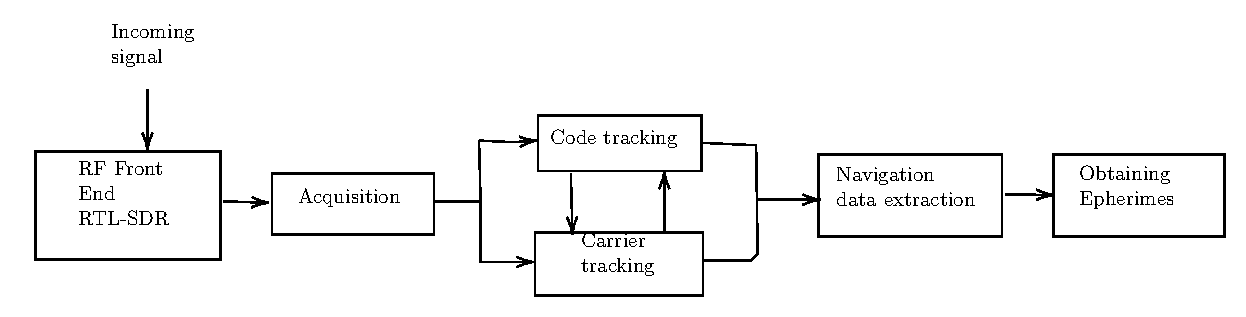
\includegraphics{figures/block2}
\end{figure} 

\end{normalsize}
\begin{Large}
\begin{center}
Figure2 : The Block Level Architecture in Demodulation
\end{center}


\subsubsection{Carrier tracking loop:}Carrier tracking loop tracks the frequency and phase of the
received signal by detecting the phase error between replicated signal and incoming signal and accordingly replicated signal produced by numerically controlled oscillator (NCO) is adjusted to synchronize with incoming signal in both frequency and phase. For zero phase error detected, navigation data is accurately extracted. Arctangent discriminator given by atan(Q/I) is used as phase
discriminator (PD) to detect phase error angle between I and Q component. Though several phase discriminators [2] are available, Atan PD has linear output over half of the input
error range (±90 0 ) and hence preferable over other types. The PD output is filtered for noise by loop filter and drives the NCO signal frequency towards the incoming carrier signal frequency.The loop filter parameters [2]: filter order, damping ratio and band width determine PLL’s ability to filter out the noise and track high signal dynamics

\subsubsection{Code tracking loop:}Post the carrier signal synchronization, received CA code samples is synchronized by aligning with replicated CA code samples by shifting right or left. To determine the direction of shift, the I and Q outputs are multiplied with prompt code (PRN code which is phase aligned), early code (prompt PRN code shifted by some samples to the right) and late code (prompt PRN code shifted by some samples to the left) resulting in corresponding to I and Q channel respectively. A code discriminator function is given by equation 4, generates error ( proportional to the code
phase error between the replica and incoming signal. This error is filtered and applied to code generator and output frequency is increased or decreased and accordingly the prompt code is phase shifted to be phase aligned with received one.
\begin{align}
\epsilon=\frac{(I^2_E+Q^2_E)-(I^2_L+Q^2_L)}{(I^2_E+Q^2_E)+(I^2_L+Q^2_L)}
\end{align}
\end{Large}\\
\begin{normalsize}
\begin{figure}[!h]%
\centering%
%\rule{30pt}{20pt}%
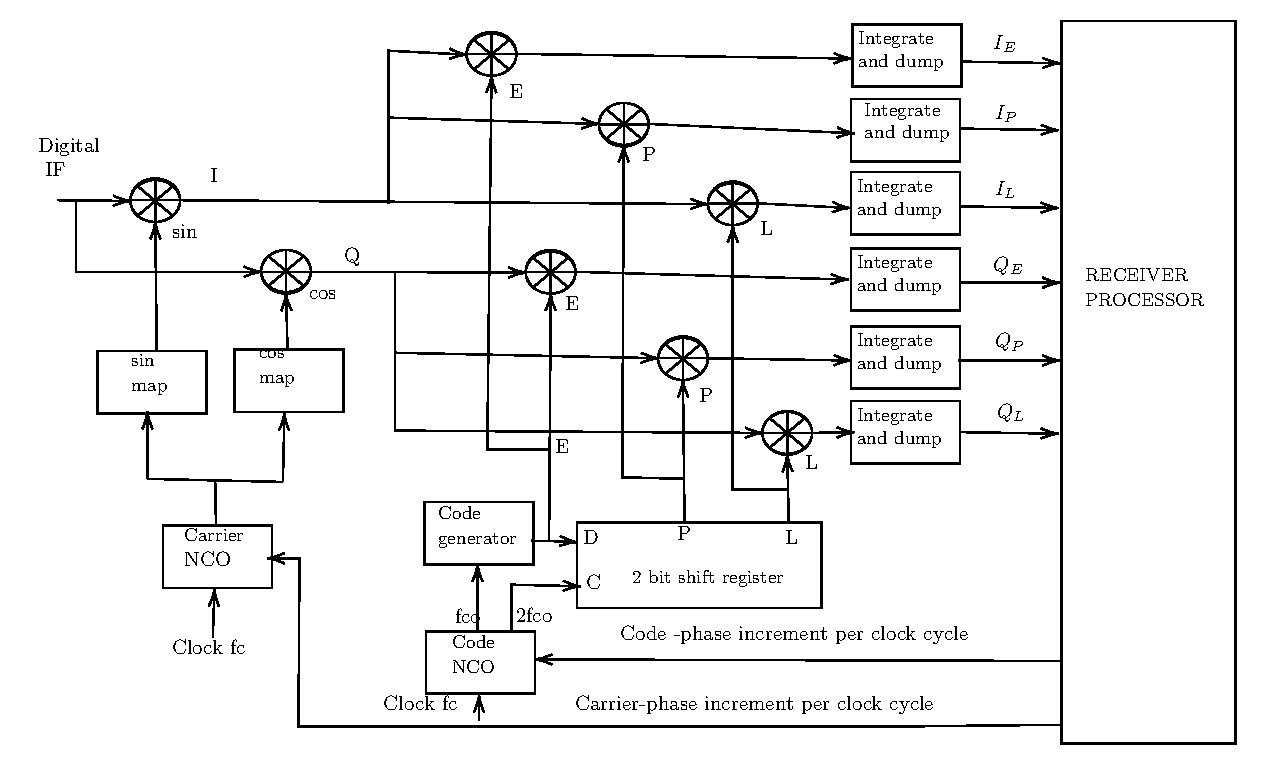
\includegraphics{figures/block3}
\end{figure}
\end{normalsize}
\begin{Large}

\begin{center}
Figure3 : Generic digital receiver channel
\end{center}
With the demodulated navigation data, the subframes can be acquired, then the ephemeris are obtained, and finally the pseudoranges as well.


\textbf{Modulation Scheme:} BPSK is a form of phase modulation where the phase of the carrier signal is shifted by 180 degrees to represent binary symbols. In NavIC, the BPSK modulation is used to modulate the navigation message, which contains important information such as satellite ephemeris, clock corrections, health status, and other navigation parameters.

\textbf{Bit Representation:} In BPSK modulation, binary 0 and 1 are represented by phase shifts of 0 degrees and 180 degrees, respectively. The navigation message in NavIC is encoded as a stream of binary bits, and each bit is mapped to a corresponding phase shift.

\textbf{Carrier Frequency:} The BPSK-modulated navigation message in NavIC is transmitted at the L5 frequency band, which is around 1176.45 MHz. This frequency is specifically allocated for satellite navigation systems.

\textbf{Data Rate:} The data rate of the BPSK-modulated navigation message in NavIC is 50 bits per second (bps). This means that the navigation message is transmitted at a rate of 50 binary bits per second.

\textbf{Error Detection and Correction:} To ensure reliable transmission, the BPSK-modulated navigation message in NavIC incorporates error detection and correction techniques. Cyclic Redundancy Check (CRC) codes are added to the navigation message, allowing the receiver to detect and correct any transmission errors.

\textbf{Symbol Synchronization:} The receiver needs to maintain synchronization with the received BPSK signal in terms of symbol timing. Synchronization algorithms are employed to detect the start of each symbol and align the demodulation process accordingly.

\subsection{Quadrature Phase Shift Keying (QPSK)}

Quadtrature phase-shift keying is widely used in digital satellite modulation. Its advantages include
strong anti-interference performance, high frequency utilization ratio and easiness to achieve. Common satellite dishes and cable television system use QPSK signal. Currently Uplink or downlink modulation of 3G and 4G standards applicable in China mostly uses QPSK. For example, channel noise threshold is as low as 4.5 dB and transmission code rate reaches 45Mb/s in digital satellite television DVB2S standard. The use of QPSK modulation guarantees both signal transmission efficiency and bit error rate performance. 

To demodulate a QPSK signal, you typically use a coherent demodulator, which consists of two parallel branches, the in-phase (I) branch and the quadrature (Q) branch. Each branch operates as a phase detector, comparing the received signal with two reference signals that are 90 degrees out of phase with each other.

The equations for demodulating a QPSK signal using a coherent demodulator are as follows:

Multiply the received signal by the in-phase reference signal (cosine wave):
\begin{align}
I_{demod} = QPSK_{rc} * \cos(2* \pi * f * t)
\end{align}

Multiply the received signal by the quadrature reference signal (sine wave):
\begin{align}
Q_{demod} = QPSK_{rc} * \sin(2* \pi * f * t)
\end{align}

Apply a low-pass filter to both $I_{demod}$ and $Q_{demod}$ to remove high-frequency components and extract the baseband signal.
\begin{align}
I_{filtered} = low\_pass\_filter (I_{demod})\\
Q_{filtered} = low\_pass\_filter (Q_{demod})
\end{align}
Sample the filtered signals at the symbol rate to obtain the demodulated data.

The demodulated data can be represented as a constellation diagram, where each point in the diagram corresponds to a specific phase shift. The receiver then determines the closest point in the constellation to recover the original data.

\subsection{Binary Offset Carrier (BOC)} 
Binary Of set Carrier-modulated signals are widely used in current and next- generation global navigation satellite systems (GNSSs). IRNSS (NavIC), Indian regional navigational satellite systems uses composite signal in which one BPSK signal with two sine BOC (5, 2) modulated signals are combined. The main idea behind using BOC modulation is to reduce the interference with BPSK modulated signal, which has a sinc shaped spectrum and have most of their spectral energy concentrated around the carrier frequency. BOC-modulated signals have low energy around the carrier frequency and spectral lobes further away from the carrier. It also helps in resisting multipath effects and other types of noise in the channel.

The demodulation process for binary phase shift keying (BPSK) and quadrature phase shift keying (QPSK) signals, which are commonly used in Binary Offset Carrier (BOC) modulation, involves mathematical equations that can be used to extract the original data from the modulated signal. Here are the demodulator equations for BOC modulation:
\subsubsection{BPSK Demodulation Equations}
BOC(1,1) BPSK modulation is a specific type of BOC modulation where the primary signal is a BPSK signal modulated onto a BOC subcarrier.
\begin{align}
r(t) = A * \cos\brak{2 \pi (f_c + f_{sub}) * t +\Phi} * s(t)
\end{align}

{\begin{table}[h]}
\centering
	\caption{\Large{Parameters Table in BOC(1,1) BPSK}}
	%%%%%%%%%%%%%%%%%%%%%%%%%%%%%%%%%%%%%%%%%%%%%%%%%%%%%%%%%%%%%%%%%%%%%%
%%                                                                  %%
%%  This is the header of a LaTeX2e file exported from Gnumeric.    %%
%%                                                                  %%
%%  This file can be compiled as it stands or included in another   %%
%%  LaTeX document. The table is based on the longtable package so  %%
%%  the longtable options (headers, footers...) can be set in the   %%
%%  preamble section below (see PRAMBLE).                           %%
%%                                                                  %%
%%  To include the file in another, the following two lines must be %%
%%  in the including file:                                          %%
%%        \def\inputGnumericTable{}                                 %%
%%  at the beginning of the file and:                               %%
%%        \input{name-of-this-file.tex}                             %%
%%  where the table is to be placed. Note also that the including   %%
%%  file must use the following packages for the table to be        %%
%%  rendered correctly:                                             %%
%%    \usepackage[latin1]{inputenc}                                 %%
%%    \usepackage{color}                                            %%
%%    \usepackage{array}                                            %%
%%    \usepackage{longtable}                                        %%
%    \usepackage{calc}                                             %%
%%    \usepackage{multirow}                                         %%
%%    \usepackage{hhline}                                           %%
%%    \usepackage{ifthen}                                           %%
%%  optionally (for landscape tables embedded in another document): %%
%%    \usepackage{lscape}                                           %%
%%                                                                  %%
%%%%%%%%%%%%%%%%%%%%%%%%%%%%%%%%%%%%%%%%%%%%%%%%%%%%%%%%%%%%%%%%%%%%%%



%%  This section checks if we are begin input into another file or  %%
%%  the file will be compiled alone. First use a macro taken from   %%
%%  the TeXbook ex 7.7 (suggestion of Han-Wen Nienhuys).            %%
\def\ifundefined#1{\expandafter\ifx\csname#1\endcsname\relax}


%%  Check for the \def token for inputed files. If it is not        %%
%%  defined, the file will be processed as a standalone and the     %%
%%  preamble will be used.                                          %%
\ifundefined{inputGnumericTable}

%%  We must be able to close or not the document at the end.        %%
	\def\gnumericTableEnd{\end{document}}


%%%%%%%%%%%%%%%%%%%%%%%%%%%%%%%%%%%%%%%%%%%%%%%%%%%%%%%%%%%%%%%%%%%%%%
%%                                                                  %%
%%  This is the PREAMBLE. Change these values to get the right      %%
%%  paper size and other niceties.                                  %%
%%                                                                  %%
%%%%%%%%%%%%%%%%%%%%%%%%%%%%%%%%%%%%%%%%%%%%%%%%%%%%%%%%%%%%%%%%%%%%%%

	\documentclass[12pt%
			  %,landscape%
                    ]{report}
       \usepackage[latin1]{inputenc}
       \usepackage{fullpage}
       \usepackage{color}
       \usepackage{array}
       \usepackage{longtable}
       \usepackage{calc}
       \usepackage{multirow}
       \usepackage{hhline}
       \usepackage{ifthen}

	\begin{document}


%%  End of the preamble for the standalone. The next section is for %%
%%  documents which are included into other LaTeX2e files.          %%
\else

%%  We are not a stand alone document. For a regular table, we will %%
%%  have no preamble and only define the closing to mean nothing.   %%
    \def\gnumericTableEnd{}

%%  If we want landscape mode in an embedded document, comment out  %%
%%  the line above and uncomment the two below. The table will      %%
%%  begin on a new page and run in landscape mode.                  %%
%       \def\gnumericTableEnd{\end{landscape}}
%       \begin{landscape}


%%  End of the else clause for this file being \input.              %%
\fi

%%%%%%%%%%%%%%%%%%%%%%%%%%%%%%%%%%%%%%%%%%%%%%%%%%%%%%%%%%%%%%%%%%%%%%
%%                                                                  %%
%%  The rest is the gnumeric table, except for the closing          %%
%%  statement. Changes below will alter the table's appearance.     %%
%%                                                                  %%
%%%%%%%%%%%%%%%%%%%%%%%%%%%%%%%%%%%%%%%%%%%%%%%%%%%%%%%%%%%%%%%%%%%%%%

\providecommand{\gnumericmathit}[1]{#1} 
%%  Uncomment the next line if you would like your numbers to be in %%
%%  italics if they are italizised in the gnumeric table.           %%
%\renewcommand{\gnumericmathit}[1]{\mathit{#1}}
\providecommand{\gnumericPB}[1]%
{\let\gnumericTemp=\\#1\let\\=\gnumericTemp\hspace{0pt}}
 \ifundefined{gnumericTableWidthDefined}
        \newlength{\gnumericTableWidth}
        \newlength{\gnumericTableWidthComplete}
        \newlength{\gnumericMultiRowLength}
        \global\def\gnumericTableWidthDefined{}
 \fi
%% The following setting protects this code from babel shorthands.  %%
 \ifthenelse{\isundefined{\languageshorthands}}{}{\languageshorthands{english}}
%%  The default table format retains the relative column widths of  %%
%%  gnumeric. They can easily be changed to c, r or l. In that case %%
%%  you may want to comment out the next line and uncomment the one %%
%%  thereafter                                                      %%
\providecommand\gnumbox{\makebox[0pt]}
%%\providecommand\gnumbox[1][]{\makebox}

%% to adjust positions in multirow situations                       %%
\setlength{\bigstrutjot}{\jot}
\setlength{\extrarowheight}{\doublerulesep}

%%  The \setlongtables command keeps column widths the same across  %%
%%  pages. Simply comment out next line for varying column widths.  %%
\setlongtables

\setlength\gnumericTableWidth{%
	100pt+%
	300pt+%
0pt}
\def\gumericNumCols{2}
\setlength\gnumericTableWidthComplete{\gnumericTableWidth+%
         \tabcolsep*\gumericNumCols*2+\arrayrulewidth*\gumericNumCols}
\ifthenelse{\lengthtest{\gnumericTableWidthComplete > \linewidth}}%
         {\def\gnumericScale{\ratio{\linewidth-%
                        \tabcolsep*\gumericNumCols*2-%
                        \arrayrulewidth*\gumericNumCols}%
{\gnumericTableWidth}}}%
{\def\gnumericScale{1}}

%%%%%%%%%%%%%%%%%%%%%%%%%%%%%%%%%%%%%%%%%%%%%%%%%%%%%%%%%%%%%%%%%%%%%%
%%                                                                  %%
%% The following are the widths of the various columns. We are      %%
%% defining them here because then they are easier to change.       %%
%% Depending on the cell formats we may use them more than once.    %%
%%                                                                  %%
%%%%%%%%%%%%%%%%%%%%%%%%%%%%%%%%%%%%%%%%%%%%%%%%%%%%%%%%%%%%%%%%%%%%%%

\ifthenelse{\isundefined{\gnumericColA}}{\newlength{\gnumericColA}}{}\settowidth{\gnumericColA}{\begin{tabular}{@{}p{100pt*\gnumericScale}@{}}x\end{tabular}}
\ifthenelse{\isundefined{\gnumericColB}}{\newlength{\gnumericColB}}{}\settowidth{\gnumericColB}{\begin{tabular}{@{}p{300pt*\gnumericScale}@{}}x\end{tabular}}

\begin{longtable}[c]{%
	b{\gnumericColA}%
	b{\gnumericColB}%
	}

%%%%%%%%%%%%%%%%%%%%%%%%%%%%%%%%%%%%%%%%%%%%%%%%%%%%%%%%%%%%%%%%%%%%%%
%%  The longtable options. (Caption, headers... see Goosens, p.124) %%
%	\caption{The Table Caption.}             \\	%
% \hline	% Across the top of the table.
%%  The rest of these options are table rows which are placed on    %%
%%  the first, last or every page. Use \multicolumn if you want.    %%

%%  Header for the first page.                                      %%
%	\multicolumn{2}{c}{The First Header} \\ \hline 
%	\multicolumn{1}{c}{colTag}	%Column 1
%	&\multicolumn{1}{c}{colTag}	\\ \hline %Last column
%	\endfirsthead

%%  The running header definition.                                  %%
%	\hline
%	\multicolumn{2}{l}{\ldots\small\slshape continued} \\ \hline
%	\multicolumn{1}{c}{colTag}	%Column 1
%	&\multicolumn{1}{c}{colTag}	\\ \hline %Last column
%	\endhead

%%  The running footer definition.                                  %%
%	\hline
%	\multicolumn{2}{r}{\small\slshape continued\ldots} \\
%	\endfoot

%%  The ending footer definition.                                   %%
%	\multicolumn{2}{c}{That's all folks} \\ \hline 
%	\endlastfoot
%%%%%%%%%%%%%%%%%%%%%%%%%%%%%%%%%%%%%%%%%%%%%%%%%%%%%%%%%%%%%%%%%%%%%%

\hhline{|-|-}
	 \multicolumn{1}{|p{\gnumericColA}|}%
	{\gnumericPB{\raggedright}\gnumbox[l]{\hspace*{1cm}\textbf{Symbol}}}
	&\multicolumn{1}{p{\gnumericColB}|}%
	{\gnumericPB{\raggedright}\gnumbox[l]{\hspace*{2cm}\textbf{Definition}}}
\\
\hhline{|--|}
	 \multicolumn{1}{|p{\gnumericColA}|}%
	{\gnumericPB{\raggedright}\gnumbox[l]{\hspace{1cm}A}}
	&\multicolumn{1}{p{\gnumericColB}|}%
	{\gnumericPB{\raggedright}\gnumbox[l]{ received signal amplitude}}
\\
\hhline{|--|}
	 \multicolumn{1}{|p{\gnumericColA}|}%
	{\gnumericPB{\raggedright}\gnumbox[l]{\hspace{1cm}$f_c$}}
	&\multicolumn{1}{p{\gnumericColB}|}%
	{\gnumericPB{\raggedright}\gnumbox[l]{carrier frequency}}
\\
\hhline{|--|}
	 \multicolumn{1}{|p{\gnumericColA}|}%
	{\gnumericPB{\raggedright}\gnumbox[l]{\hspace{1cm}$f_{sub}$}}
	&\multicolumn{1}{p{\gnumericColB}|}%
	{\gnumericPB{\raggedright}\gnumbox[l]{subcarrier frequency (which is half the chip rate)}}
\\
\hhline{|--|}
	 \multicolumn{1}{|p{\gnumericColA}|}%
	{\gnumericPB{\raggedright}\gnumbox[l]{\hspace{1cm}t}}
	&\multicolumn{1}{p{\gnumericColB}|}%
	{\gnumericPB{\raggedright}\gnumbox[l]{time}}
\\
\hhline{|--|}
	 \multicolumn{1}{|p{\gnumericColA}|}%
	{\gnumericPB{\raggedright}\gnumbox[l]{\hspace{1cm}q}}
	&\multicolumn{1}{p{\gnumericColB}|}%
	{\gnumericPB{\raggedright}\gnumbox[l]{ phase offset}}
\\
\hhline{|--|}
	 \multicolumn{1}{|p{\gnumericColA}|}%
	{\gnumericPB{\raggedright}\gnumbox[l]{\hspace{1cm}s(t)}}
	&\multicolumn{1}{p{\gnumericColB}|}%
	{\gnumericPB{\raggedright}\gnumbox[l]{BPSK signal transmitted data(-1,1)}}
\\
\hhline{|-|-|}
\end{longtable}

\ifthenelse{\isundefined{\languageshorthands}}{}{\languageshorthands{\languagename}}
\gnumericTableEnd

{\end{table}}
To demodulate the BOC(1,1) BPSK signal, we need to multiply the received signal by the carrier wave and then integrate it over one chip duration $(T_{chip}).$ The demodulated signal is given by:
\begin{align}
y(t) = \int[r(t) * \cos(2\pi(f_c + f_{sub}) * t + \Phi)] dt
\end{align}
\begin{align}
= \frac{A}{2} * s(t) * \cos(2\pi(f_c + f_{sub}) * t + \Phi)
\end{align}
To recover the original data, we compare the demodulated signal with a threshold value. If y(t) > 0, the transmitted data is +1; otherwise, it is -1.
\subsubsection{QPSK Demodulation Equations}
BOC(1,1) QPSK modulation is another type of BOC modulation where the primary signal is a QPSK signal modulated onto a BOC subcarrier.I(t) is the in-phase component of the QPSK signal, which can be represented as +1 or -1 depending on the transmitted data, and Q(t) is the quadrature component of the QPSK signal, which can also be represented as +1 or -1 depending on the transmitted data.
\begin{align}
r(t) = A * \cos(2\pi(f_c + f_{sub}) * t + \Phi) * I(t) * Q(t)
\end{align}
To demodulate the BOC(1,1) QPSK signal, we need to multiply the received signal by both the in-phase and quadrature carriers and then integrate them over one chip duration $(T_chip)$. The demodulated in-phase and quadrature signals are given by:
\begin{align}
y_{I(t)} = \int\sbrak{r(t) * cos(2\pi(f_c + f_{sub}) * t + \Phi) * cos(2\pi(f_c + f_{sub} * t)} dt\\
= \frac{A}{2} * I(t) * cos(2\pi(f_c + f_{sub}) * t + \Phi)\\
y_{Q(t)} = \int\sbrak{r(t) * cos(2\pi(f_c + f_{sub}) * t + \Phi) * sin(2\pi(f_c + f_{sub}) * t)} dt\\
= \frac{A}{2} * Q(t) * cos(2\pi(f_c + f_{sub}) * t + \Phi)
\end{align}
To recover the original data, we compare the demodulated in-phase $(y_{I(t)})$ and quadrature $(y_{Q(t)})$ signals with a threshold value. The transmitted data can be determined based on the combinations of I(t) and Q(t).
\end{Large}

\end{enumerate}
\end{document}
